\documentclass[12pt]{article}
%\usepackage[utf8]{inputenc}
%\documentclass[UTF8]{ctexart}
%\usepackage[UTF8, heading = false, scheme = plain]{ctex}
\usepackage{geometry}
%geometry{a4paper,scale=0.9}
\geometry{a4paper,left=1cm,right=1cm,top=1cm,bottom=2cm}
\usepackage{amsfonts}
\usepackage{color}
\usepackage{url}
%\usepackage{biblatex}
\usepackage{amsmath}
\usepackage{amssymb}
\usepackage{latexsym}
\usepackage{cite}
%\addbibresource{ref.bib}
%\bibliography{ref.bib}
\usepackage{caption}
\usepackage{graphicx, subfig}
\usepackage{float}
%\usepackage[fontset=ubuntu]{ctex}
%\usepackage{fontspec}
\usepackage{xeCJK}
%\usepackage[colorlinks,
%anchorcolor=black,
%citecolor=black]{hyperref}
%\setmainfont{SimSun}
\usepackage[section]{placeins}
\usepackage{enumitem}
\usepackage{framed}
\usepackage[framemethod=TikZ]{mdframed}
\usepackage{indentfirst}
\usepackage{setspace}%使用间距宏包
\linespread{1.5}
%\title{预备知识}
%\author{leolinuxer }
%\date{June 2020}

\title{Lambdamart 介绍\cite{A_Not_So_Simple_Introduction_To_Lambdamart}}
\author{leolinuxer}
%\date{June 2020}

\begin{document}
\maketitle
\tableofcontents

\section{Lambdamart 简介}
在排序问题中使用的机器学习算法,被称为 Learning to Rank (LTR) 算法,或者 Machine-Learning Rank (MLR) 算法。

LTR 算法通常有三种手段,分别是:Pointwise、Pairwise 和 Listwise。Pointwise 和 Pairwise 类型的 LTR 算法,将排序问题转化为回归、分类或者有序分类问题。Listwise 类型的 LTR 算法则另辟蹊径,将用户查询(Query)所得的结果作为整体,作为训练用的实例(Instance)。

LambdaMART 是一种 Listwise 类型的 LTR 算法。
它基于 LambdaRank 算法和 MART (Multiple Additive Regression Tree) 算法,将\textbf{搜索引擎结果排序问题转化为回归决策树问题}。

\textbf{MART 实际就是梯度提升决策树(GBDT, Gradient Boosting Decision Tree)算法}。GBDT 的核心思想是在不断的迭代中,新一轮迭代产生的回归决策树模型拟合损失函数的梯度,最终将所有的回归决策树叠加得到最终的模型。

\textbf{LambdaMART 使用一个特殊的 Lambda 值来代替上述梯度,也就是将 LambdaRank 算法与 MART 算法加和起来}。考虑到 LambdaRank 是基于 RankNet 算法的,所以在搞清楚 LambdaMART 算法之前,我们首先需要了解 MART、RankNet 和 LambdaRank 是怎么回事。

\section{MART 算法}
MART,即多重增量回归树(Multiple Additive Regression Tree)有许多名字:
\begin{itemize}
\setlength{\itemsep}{0pt}
\setlength{\parsep}{0pt}
\setlength{\parskip}{0pt}
    \item MART - 多重增量回归树(Multiple Additive Regression Tree)
    \item GBDT - 梯度渐进决策树(Gradient Boosting Decision Tree)
    \item GBRT - 梯度渐进回归树(Gradient Boosting Regression Tree)
    \item TreeNet - 决策树网络(Tree Net)
\end{itemize}

这些名字的含义都一样,都是一个意思。从这些名字,我们可以看出 MART 的一些特征:
\begin{itemize}
\setlength{\itemsep}{0pt}
\setlength{\parsep}{0pt}
\setlength{\parskip}{0pt}
    \item 使用决策树来预测结果;
    \item 用到的决策树有很多个;
    \item 每个树都比之前的树改进一点点,逐渐回归、拟合到真实结果。
\end{itemize}

实际上,这三点是 Boosting 思想的精髓。

\section{Boosting(渐进)思想}
Boosting 思想,尝试通过不断迭代弱模型(Weak Learner),通过叠加弱模型的方式,渐进地逼近真实情况,起到足以预测真实值的强模型的作用。显而易见,Boosting 思想至少需要解决两个问题:
\begin{itemize}
\setlength{\itemsep}{0pt}
\setlength{\parsep}{0pt}
\setlength{\parskip}{0pt}
    \item 如何保证每一次迭代都对解决问题有所帮助,或者说如何确定迭代步骤中拟合的方向?
    \item 如何将每一次迭代产生的弱模型有效地叠加起来?
\end{itemize}

下面,我们通过 AdaBoost(Adaptive Boosting,自适应渐进法)来回答这两个问题。

\section{AdaBoost}
AdaBoost 是一种用于分类的算法,它的运行过程大致可以理解如下:
\begin{enumerate}
\setlength{\itemsep}{0pt}
\setlength{\parsep}{0pt}
\setlength{\parskip}{0pt}
    \item 制作一个弱分类器(实际是一个决策树),去拟合实际情况,我们将它记录为 $WL_1$;
    \item 运行 $WL_1$,记录分类错误的那些样本。接下来,赋予这些被错误分类的样本比较高的权重,进行第二次拟合,得到新的弱分类器 $WL_2$;
    \item 依次运行 $WL_1 - WL_2$,记录分类错误的那些样本。接下来,赋予这些被错误分类的样本比较高的权重,进行第三次拟合,得到新的弱分类器 $WL_3$;
    \item 依次运行 $WL_1 - WL_2 - WL_3$,如此迭代……
\end{enumerate}

下图是讲述的是运用 Boosting 思想进行分类的过程。蓝色和红色的圆圈,代表两类样本,圆圈的大小代表当前该点的权重;绿色的线条代表训练既得分类器模型;虚线表示当前训练新增的分类器模型。可以看到,在不断的迭代过程中,每一次迭代,分类器都会关注之前区分错误的那些样本点,进行有针对性的处理。因此,在进行到 150 次迭代之后(m=150),最终叠加起来的模型已经非常细致,足够将红蓝两种类别细致地区分开来了。
\begin{figure}[H]
\centering
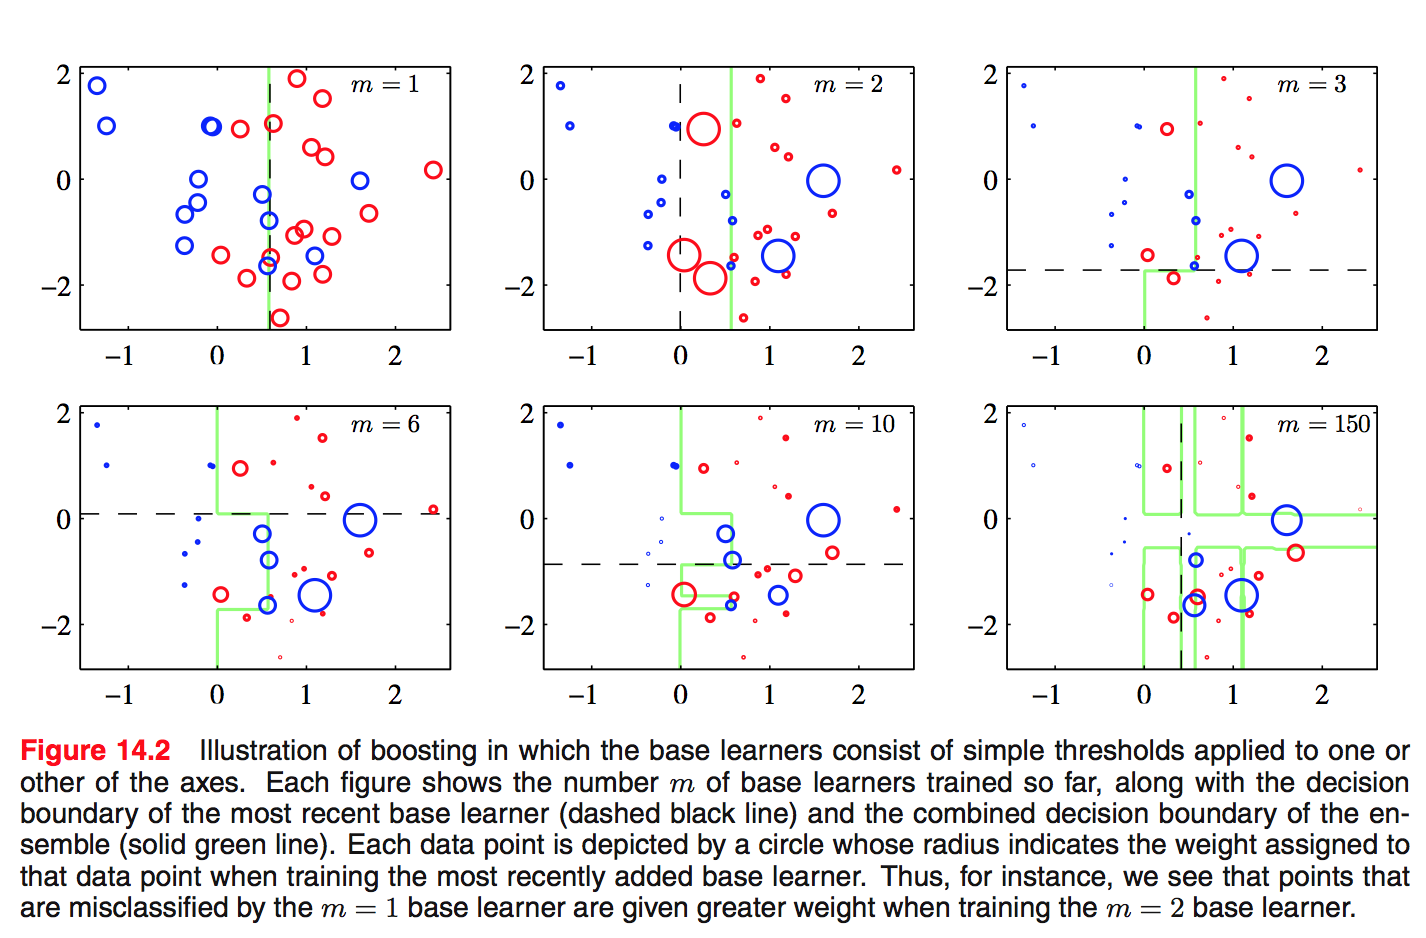
\includegraphics[width=.8\textwidth]{fig/boosting_example.png} 
\end{figure}

整个过程,用数学符号表达如下:
\begin{figure}[H]
\centering
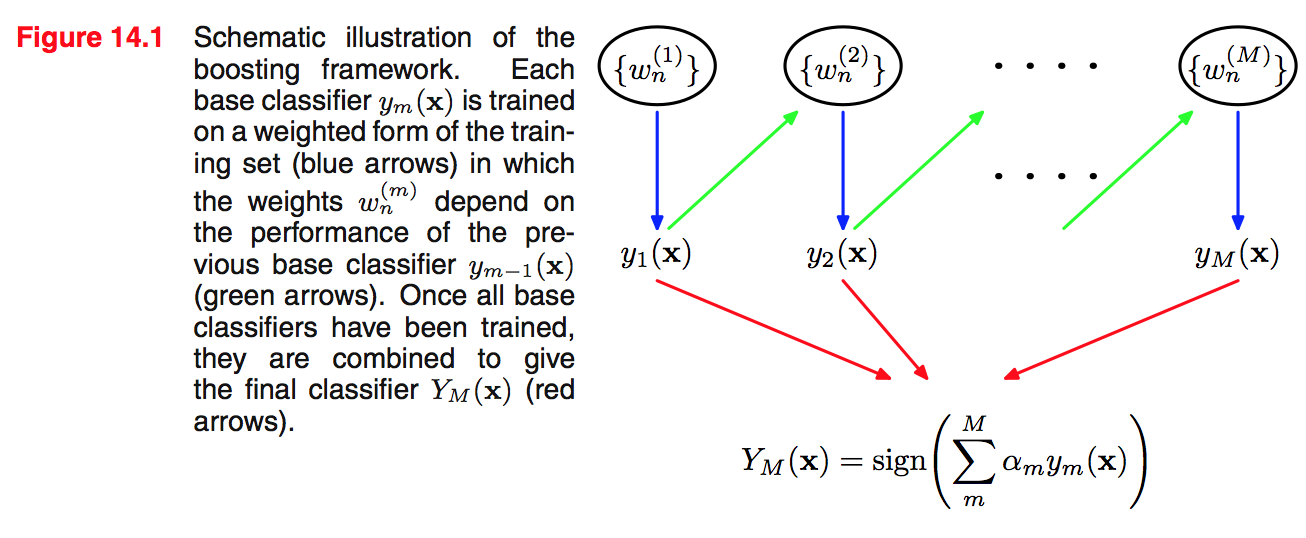
\includegraphics[width=.8\textwidth]{fig/boosting_process.png} 
\end{figure}

符号解释:
\begin{itemize}
\setlength{\itemsep}{0pt}
\setlength{\parsep}{0pt}
\setlength{\parskip}{0pt}
    \item $w_n^{k}$表示一个$n$元向量,向量中的每一个元素都对应训练集中的一个样本点;向量中元素的值,就是所对应样本点在第$k$次迭代中的权重;
    \item $y^k(x)$ 是根据上述权重计算出来的第$k$ 次迭代的模型;
    \item  $\alpha_k$是第$k$次迭代的模型的权重;
    \item $Y_M(x)$是根据上述 $M$ 个弱分类器加权求和得到的最终分类器。
\end{itemize}

最开始的时候,每个样本点的权重都一致。随着算法不断迭代,被错误分类的样本,权重不断加强,与此同时被正确分类的样本,权重不断减弱。可以想象,越往后,算法越关注那些容易被分错的样本点,从而最终解决整个问题。

因此,从 AdaBoost 的角度可以回答 boosting 算法要解决的两个问题:
\begin{itemize}
\setlength{\itemsep}{0pt}
\setlength{\parsep}{0pt}
\setlength{\parskip}{0pt}
    \item AdaBoost 通过调整样本的权值,来确定下一轮迭代中弱模型的拟合方向:提升分类错误的样本的权值,降低分类正确的样本的权值。
    \item AdaBoost 用一个「加法模型」,将每一轮迭代得到的弱模型组合叠加起来,得到一个有效的强模型。
\end{itemize}

\section{MART 的数学原理}
MART 是一种 Boosting 思想下的算法框架,它的目标是寻找强模型$f(x)$满足:
$$
\hat{f}(x) = \arg\min_{f(x)} = E[L(y,f(x))|x]
$$

和 AdaBoost 一样,训练之后的 MART 模型也是一个加法模型,形式如下:
$$
\hat{f}(x) = \hat{f}_M(x) = \sum_{m=1}^Mf_m(x)
$$

这里:
\begin{itemize}
\setlength{\itemsep}{0pt}
\setlength{\parsep}{0pt}
\setlength{\parskip}{0pt}
    \item $\hat{f} = \hat{f}_M: \mathbb{R}^d \mapsto \mathbb{R}$ 是模型的目标函数;
    \item $x \in \mathbb{R}^d$ 是样本点,它包含  $d$个特征的值;
    \item $\hat{f}(x) \in \mathbb{R}$ 是预测值;
    \item $M$ 是训练过程中迭代的次数,也就是模型中回归决策树的数量;
    \item $f_m: \mathbb{R}^d \mapsto \mathbb{R}$ 是模型训练过程中得到的弱模型(也就是回归决策树)。
\end{itemize}

那么,关于 MART 的 Boosting,我们还剩下一个回答,即:如何保证每一次迭代都对解决问题有所帮助,或者说如何确定迭代步骤中拟合的方向。接下来的分析,我们就来解决这个问题。

假设我们已经迭代了$m$次,得到了$m$颗决策树。我们将这$m$  颗决策树的和记作 $\hat{f}_m(x) = \sum_{i=1}^mf_i(x)$
,于是,第 $i+1$ 轮拟合的目标:
$$
\delta \hat{f}(x)_{m+1} = \hat{f}(x)_{m+1} - \hat{f}(x)_{m} = f_{m+1}
$$

现在我们要求这个 $\delta \hat{f}(x)_{m+1}$
。我们引入损失函数:
$$
L = L((x,y),f) = L(y,f(x)|x)
$$

来描述预测函数$f$的预测结果$y^*=f(x)$与真实值
$y$的差距。那么,我们的目的是要在进行第 $m+1$ 轮拟合之后,预测值与真实情况的差距会减小,即:
$$
\delta L_{m+1} = L((x,y),\hat{y}_{m+1}) - L((x,y),\hat{f}_m) < 0
$$

考虑到:
$$
\delta L_{m+1} \approx \frac{\partial L((x,y),\hat{f}_m)}{\partial \hat{f}_m} \cdot \delta \hat{f}_{m+1}
$$

\bibliography{../ref}
\bibliographystyle{IEEEtran}
\end{document}
